\documentclass{article}
\usepackage[utf8]{inputenc}
\usepackage{preamble}
\usepackage{subcaption}
\usepackage{caption}
%\usepackage{siunitx}
%\usepackage{physics}
\newcommand{\vecS}{\boldsymbol{\vec{S}}}
\usepackage{amsthm}
\usepackage{hyperref}
\usepackage{cleveref}
\newtheoremstyle{indented}{3pt}{3pt}{\addtolength{\leftskip}{1.5em}\addtolength{\rightskip}{1.5em}}{}{\bfseries}{.}{.5em}{}

\theoremstyle{indented}
\newtheorem{definition}{Definition}
\newtheorem{example}{Example}
\newtheorem{proposition}{Proposition}
\newcommand{\evec}{\boldsymbol{\hat{e}}}
\newcommand{\image}{\operatorname{im}}
\newcommand{\aut}{\operatorname{Aut}}

\begin{document}

\begin{center}
   \LARGE{\textsc{MATH 271, Project}}\\
   \large{\textsc{Due December 18$^\textrm{th}$}}
\end{center}
\vspace{.5cm}

\section*{Due Date}
The assignment must be turned in via Canvas by Friday December 18$^\textrm{th}$, 2020, by 11:59PM mountain time.
\subsection*{Requirements}
\begin{itemize}
    \item You may work together, but you must submit your own individual work.
    \item You are to type out your work to this assignment using a program like Microsoft Word or \LaTeX. If you use a program like Microsoft Word, use the equation editor for any mathematical symbols you use.
    \item Save your document as a PDF as only PDF files will be accepted. Make sure your formatting comes out correctly when you save as a PDF! Microsoft Word has a way of making this more challenging than it needs to be.
    \item For full credit, explain your work along the way and use consistent notation.  Though problems may not ask for much, a short and complete explanation is expected.
\end{itemize}

Just as a remark, words written in blue are emphasized since they are either definitions or common terms used in mathematics that I may not define explicitly here. Also, there are 15 total problems.

\section{Introduction}

Before doing anything, I'm opening this up to a problem for you.

\begin{problem}{}{}
In chemistry or in your area of research interest, is group theory used? If so, what are the applications of group theory? Do those applications have any interest to you?
\end{problem}

Let us begin this with a motivating question rather than a mathematical definition.\\

\noindent \textbf{Question:} Given a set $S$, possibly with some structure, what is the set of symmetries $G$ of this set?\\

Nature loves symmetry. If you spend any time looking at the world around you, you will find highly symmetric objects. Some of these objects are beautiful and coveted by us humans.

\begin{figure}[H]
    \centering
\begin{subfigure}[b]{0.3\textwidth}
    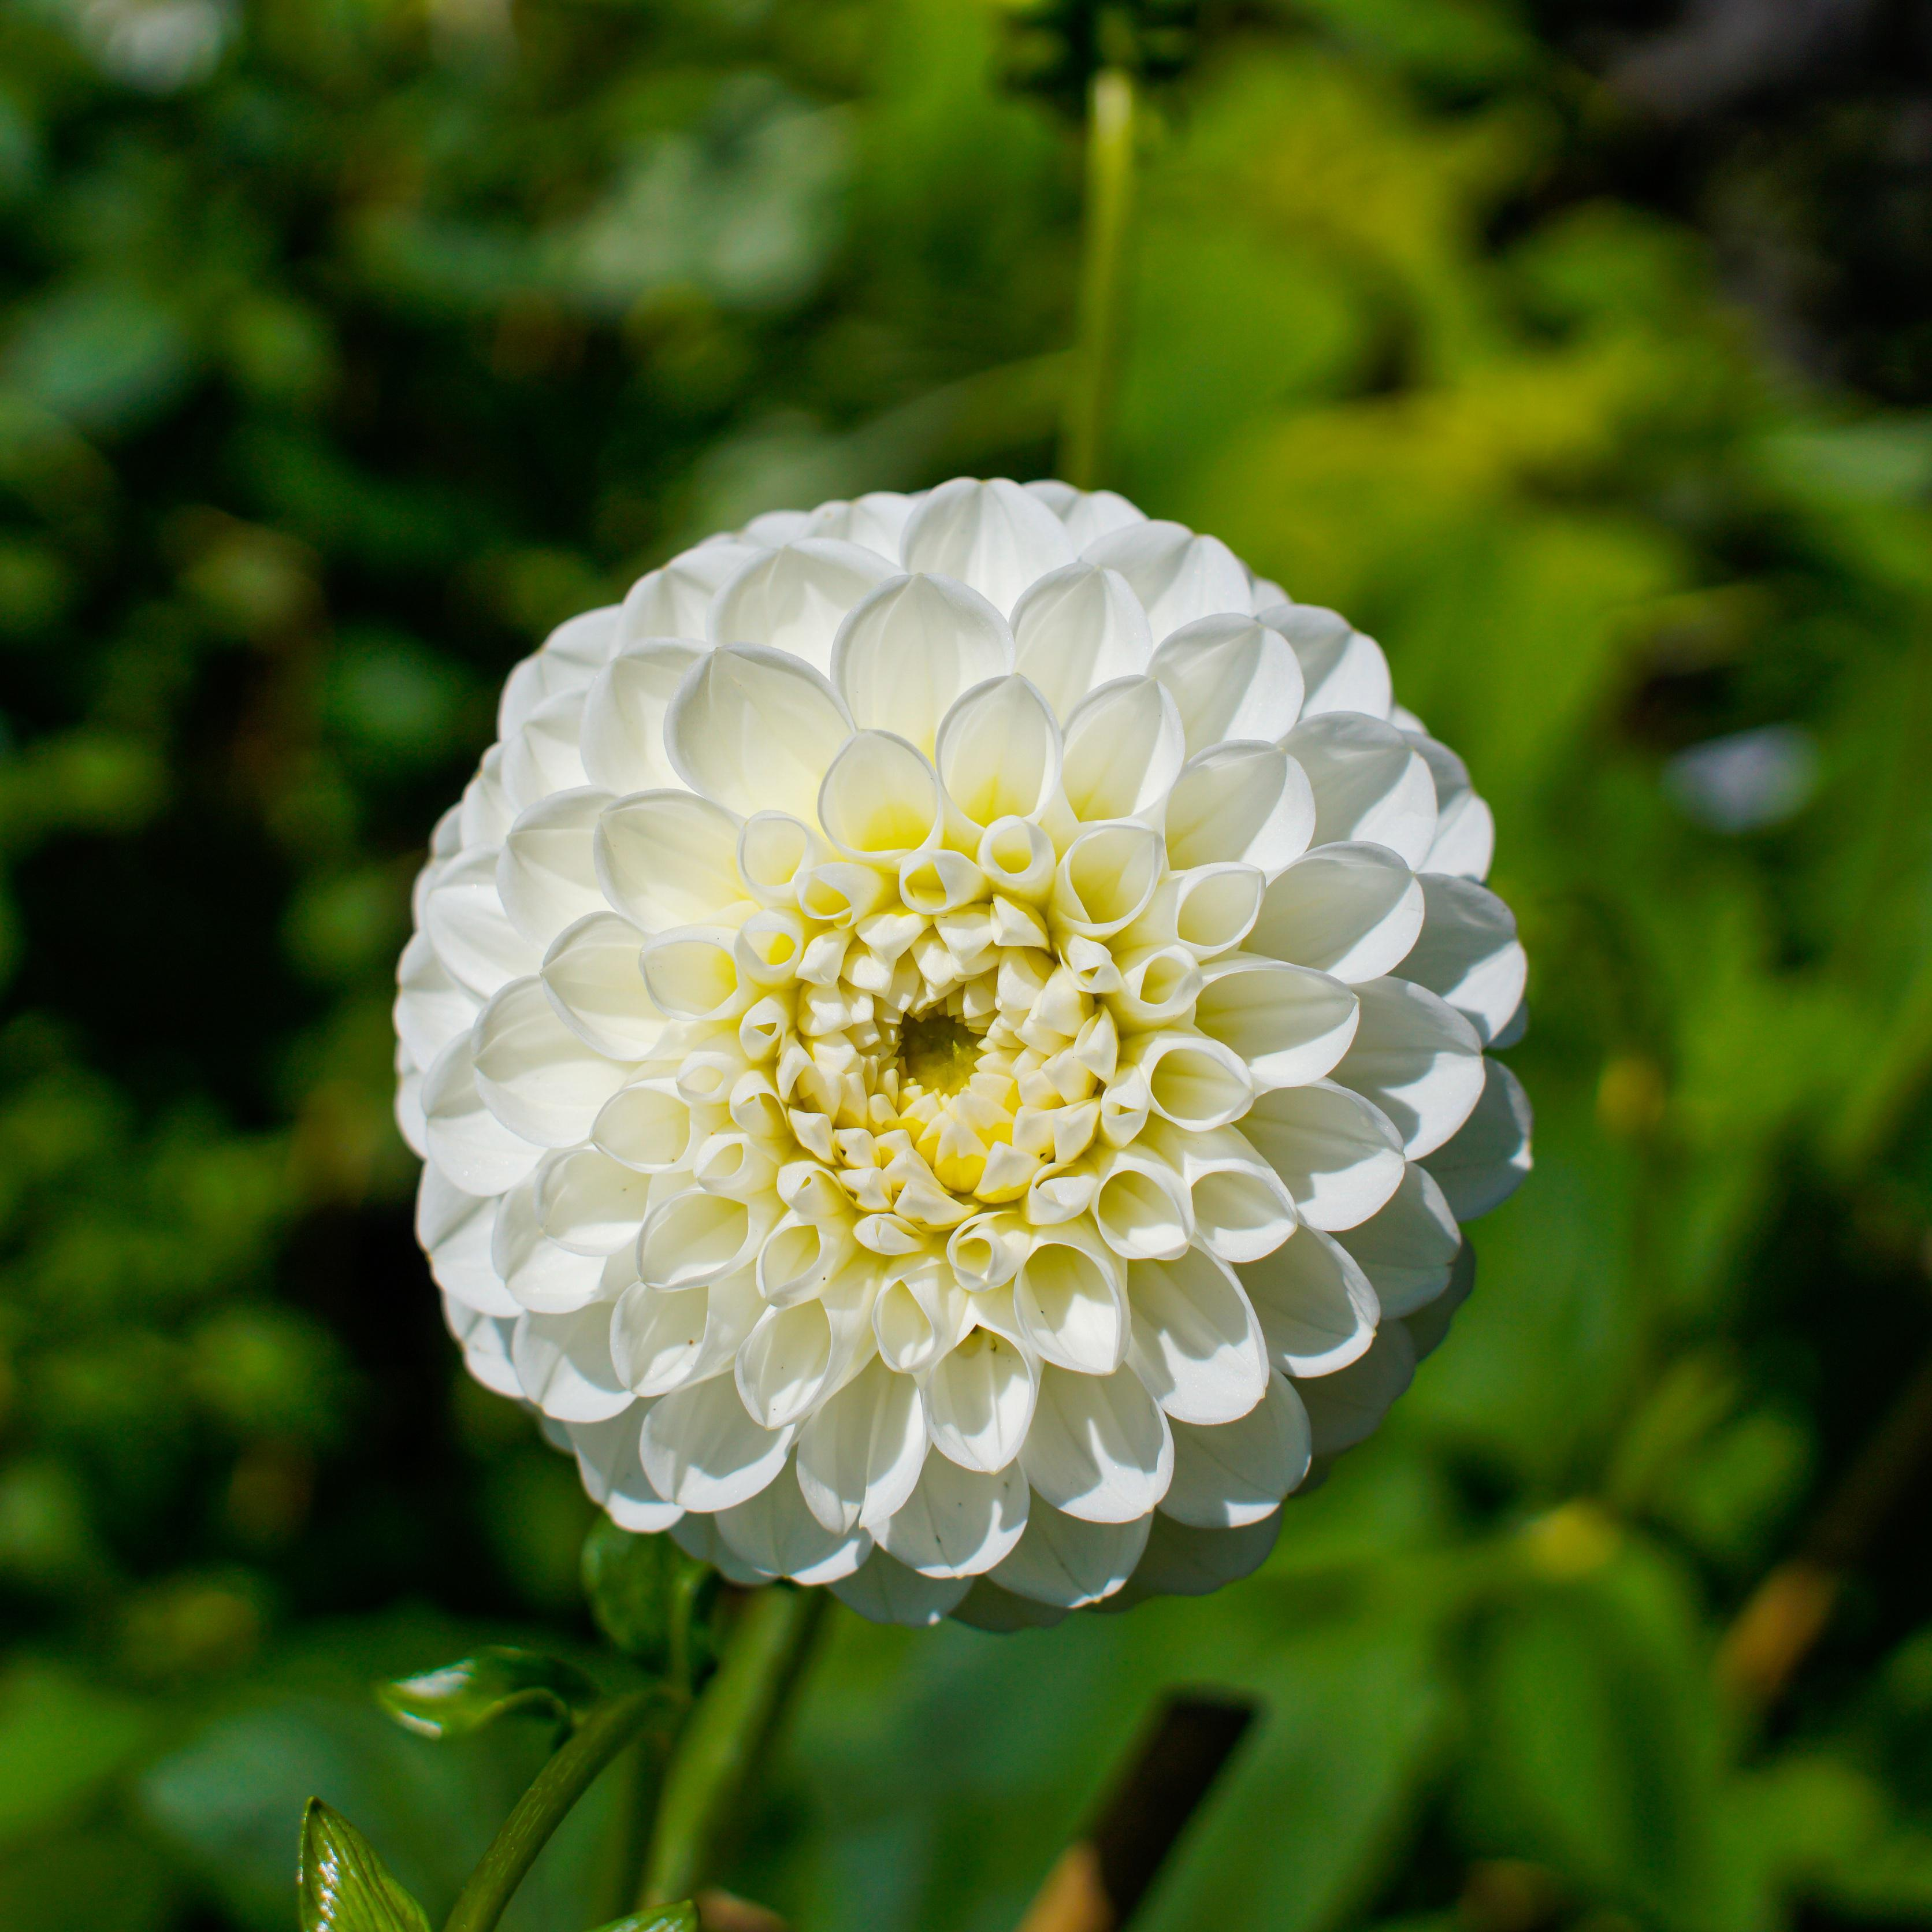
\includegraphics[width=\textwidth]{symmetric_flower.jpg}
\end{subfigure}
\qquad \qquad \qquad
\begin{subfigure}[b]{0.3\textwidth}
    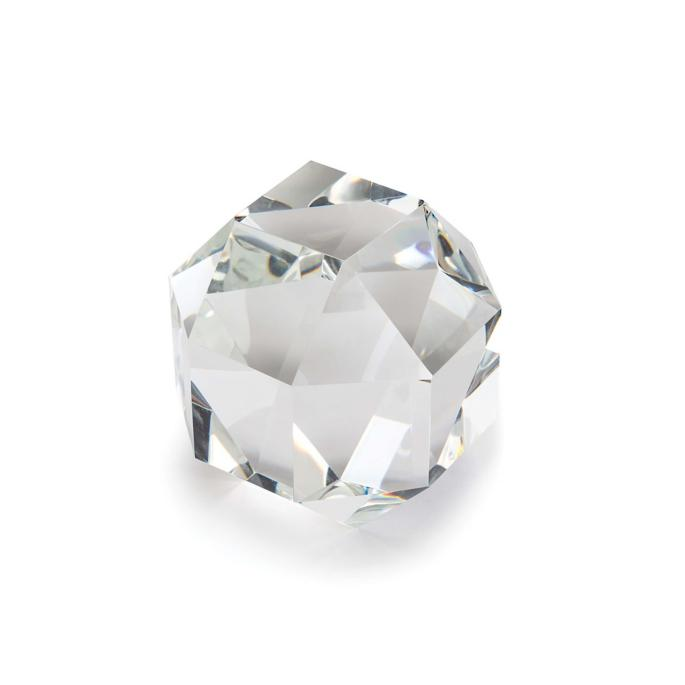
\includegraphics[width=\textwidth]{symmetric_diamond.jpg}
\end{subfigure}
\end{figure}

We now need to be precise. What exactly does it mean to be a symmetry of a set? Physically, a symmetry is something we see with objects. A concrete example would be a square sheet of paper. If we lay a square sheet of paper on a desk, you could leave the room, another person could move this paper, and if you came back, you would not notice this change. This is a symmetry. If the move remains undocumented, no one can tell the difference. As a scientist, you would like to document these changes so you prepare the experiment better. You label the corners of the square $A$, $B$, $C$, and $D$. Then, you place a pin in the center of the square at the origin $0$ so that the paper cannot be picked up. Then you could only record the following symmetries.

\begin{figure}[H]
    \centering
    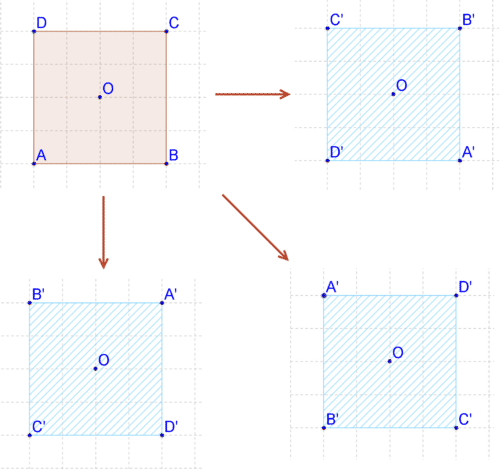
\includegraphics[width=.75\textwidth]{square_rotations.jpg}
\end{figure}

One can imagine a situation with a more complicated object. Some objects may be too complicated to have much symmetry. There seems to be a balance here. In the example with the square, we restricted ourselves a bit. By placing a pin at $0$, we forbid the paper from lifting, but did this lose us some extra symmetries of flipping the paper? Sure. If instead, we made a pentagon, do we expect more symmetries or less? A triangle? What about a rectangle? What is the right way to encode symmetries of all objects mathematically such that these ideas of restrictions and generalizations behave properly?

Sticking with pinned down square, let's notice some things. Any rotation can be applied after any rotation which means we can \boldblue{compose} symmetries. We can \boldblue{invert} any symmetry by rotating in the opposite direction. In fact, with this example, we can \boldblue{generate} all possible symmetries by rotating the square by $\pi/2$ in the counterclockwise direction. The last fact is rather special.

Now, our goal is to make all of this mathematical. You may ask why, and that's a fair question. The reason why is to give ourselves a well-defined toolbox to tackle any problem where symmetry is involved. Mathematics provides us truth by logic. We may be able to realize even more powerful statements, classify symmetries, and utilize them in areas such as physics, chemistry, biology, computer science, or even art.

\section{Mathematics of Symmetries}

As we began, fix any set $S$. This set may contain or represent whatever it is you need at the moment. For now, we let it be arbitrary. An action on this set is given by a function $f\colon S \to S$. A symmetry does not distort the set, so we cannot do anything malicious such as delete members under some symmetry operation. That greatly restricts our choice of such actions.

\begin{definition}
A \boldblue{symmetry action} on a set $S$ is a function $f\colon S \to S$ such that $f$ is one-to-one (injective) and onto (surjective). Equivalently, an injective and surjective function is called a bijection.
\end{definition}

\begin{example}
\label{ex:s3}
Let $S = \{A,B,C\}$, then there are $3!=6$ symmetry actions of $S$. That is, this is the number of ways to rearrange a set of size $S$ (can you prove this?). We can define a bijective function $f\colon S \to S$ by choosing what it does to each input, so we will write $f(A,B,C)$ all at once. Here is the list, in no particular order:
\begin{align*}
    f_0(A,B,C) &= (A,B,C)\\
    f_1(A,B,C) &= (B,A,C)\\
    f_2(A,B,C) &= (A,C,B)\\
    f_3(A,B,C) &= (C,B,A)\\
    f_4(A,B,C) &= (B,C,A)\\
    f_5(A,B,C) &= (C,A,B)
\end{align*}
The set of all symmetry actions of $S$ is the set
\[
G = \{f_0,f_1,f_2,f_3,f_4,f_5\}.
\]
This set $G$ is well known. It is typically called the \boldblue{symmetric group on 3-elements} and we use the notation $S_3\coloneqq G$.

For sake of clarity, a non-example would be a function $g\colon S \to S$ whereby
\[
g(A,B,C) = (A,A,C).
\]
This function is not injective since we have that $A\mapsto A$ and $B\mapsto A$ and it is not surjective since $B$ is not in the image of $g$.
\end{example}

This set $S$ in \cref{ex:s3} was given no additional structure like the geometry we imposed with the square. In that case, the geometry dictated that we must take more care when speaking of symmetries. We even pinned the square down and reduced the number of symmetries further. Let's investigate this.

\begin{example}
\label{ex:square_c}
To model our points of a square, let us work with the square in the complex plane $\C$ for sake of ease. Let $S=\{1,i,-1,-i\}\subset \C$ be the vertices of the square. Then, all valid rotational symmetry actions must be integer copies of $n\frac{\pi}{2}$ where rotations of $S$ are given by multiplication by $e^{in\frac{\pi}{2}}$. For example, take $n=1$, then $e^{i\frac{\pi}{2}}=i$. Let $f_{\frac{\pi}{2}}\colon S \to S$ be given by
\[
f_{\frac{\pi}{2}}(s) = is.
\]
Then,
\begin{align*}
f_{\frac{\pi}{2}}(1) &= i\\
f_{\frac{\pi}{2}}(i) &= -1\\
f_{\frac{\pi}{2}}(-1) &= -i\\
f_{\frac{\pi}{2}}(-i) &= 1.
\end{align*}
Using this notation, we can realize that $f_0=f_{2\pi}$, so the valid choices are $n=0,1,2,3$. That is, rotation by $0$, $\pi/2$, $\pi$, and $3\pi/2$. The set of symmetry actions is
\[
G= \{f_{0},f_{\frac{\pi}{2}}, f_{\pi}, f_{\frac{3\pi}{2}}\}.
\]
Amazingly, this set $G$ corresponds to the set $S$ itself since $f_{\frac{\pi}{2}}$ is just multiplication by $i$. What I mean is that,
\[
i^2=-1,\qquad i^3=-i, \qquad i^4 = 1,\qquad i^5=i
\]
and just by taking powers of $i$ we generated the set $S$. Furthermore, you may recall that this set $S$ are the set of roots to the equation
\[
z^4=1,
\]
otherwise called the $4^\textrm{th}$ roots of unity.
\end{example}

Even in the previous example it becomes apparent that there will be more than one way to address symmetries. Sometimes the underlying set itself contains enough information to build its own symmetries. In other words, we may not need to think of functions on the set for every example. However, the next example will show us that sometimes we have to and it depends on the set we start with.

\begin{example}
\label{ex:square_r2}
Perhaps it is easier to think of points of a square as vectors in $\R^2$. This is no different than using $\C$, but this goes to show that there is more than one way to \boldblue{represent} symmetries but they will always reduce to symmetry actions on a set. Let $\evec_1,\evec_2$ be the standard orthonormal basis for $\R^2$ and define the set
\[
S= \left\{\evec_1,\evec_2, -\evec_1, -\evec_2 \right\}.
\]
Then the linear transformation $J\colon \R^2 \to \R^2$ given by $J(\evec_1)=\evec_2$ and $J(\evec_2)=-\evec_1$ is a symmetry action of this set which corresponds to rotation by $\pi/2$ in the counterclockwise direction. You have shown in your homework that this $J$ corresponds to multiplication by $i$, so this should not be a surprise.

Using the fact that rotation by $\pi/2$ generates all possible rotations of the square, we have
\[
G=\{I,J,J^2,J^3\},
\]
where $I$ is the identity transformation. You can note as well that $J^2=-I$ and $J^3=-J$, if you'd like.

We also built a way to work with matrices as linear transformations for which we have
\[
[J] = \begin{pmatrix} 0 & -1 \\ 1 & 0 \end{pmatrix}
\]
in the standard orthonormal basis. This is another representation, and you can show using the same homework problems that $[J]^2=-[I]$, $[J]^3=-[J]$ and $[J]^4 = [I]$. In fact, the notation with the brackets was just a method of converting data. Applying the brackets $[]$ to $J$ just yields the matrix for $J$ in the standard basis. To that end, we could have written $[J^2]=[J]^2$ all along.
\end{example}

These past two examples have been given in terms of concrete sets whose objects we have an inherent understanding of. Complex numbers are points in a plane as vectors in $\R^2$ are arrows in a plane based at the origin. Finally, we consider the same underlying symmetries but from the perspective of an abstract concept called a \boldblue{presentation}.

\begin{example}
\label{ex:c4}
Define the following: Let $G$ be a set containing $g$ and let $G$ act on itself via a binary operation $G\times G \to G$ which we write as concatenation. That is, given $g,h\in G$ we have $(g,h)\mapsto gh$ is some potentially different element in $g$. This is no different to how we write $xy$ as a product when $x,y\in \R$.

Then we define $gg=g^2$ and add in the additional \boldblue{relation} that $g^4=e$. This $e$ is called the \boldblue{identity} and we have for any $g\in G$ that $eg=ge=g$. Then,
\[
G=\{e,g,g^2,g^3\}.
\]
This looks no different than \cref{ex:square_r2} as we have replaced $J$ with $g$. But, with this set $G$, we have assumed no extra structure aside from the relation $g^4=e$. In fact, we write this succinctly as
\[
G\coloneqq \langle g ~|~ g^4=e \rangle
\]
which is read ``$G$ is presented as the group generated by the element $g$ with the relation that $g^4$ is the identity element $e$". This object $G$ is also well known. Usually, it is called the \boldblue{cyclic group of order $4$} and is denoted by $C_4\coloneqq G$.
\end{example}

\section{Groups}

Though \cref{ex:square_c,ex:square_r2,ex:c4} represent the symmetries of the square using different structures, we would like to think of these as models of the same underlying symmetry principle. This is a big motivation for a more rigorous mathematical interpretation. \cref{ex:c4} turns out to be the way to go.

\begin{definition}
    Let $G$ be a set. Then $G$ is a \boldblue{group} if the following are satisfied.
    \begin{enumerate}[i.]
        \item $G$ has an associative binary operation $G\times G \to G$. That is, given $g,h,p \in G$, $(gh)p = g(hp)= ghp$. Here we are writing the product as concatenation.
        \item There exists an identity element $e \in G$ such that for all $g\in G$, $eg=ge=g$.
        \item For all $g\in G$, there exists $g^{-1}$ so that $gg^{-1}=g^{-1}g = e$.
    \end{enumerate}
\end{definition}

\begin{problem}{}{}
Show that the examples before are groups.
\end{problem}

\begin{problem}{Dihedral group}{}
The full symmetries of the square are captured by the dihedral group $D_4$ (sometimes written $D_{8}$). This group is presented by
\[
D_4 = \langle r,s ~\vert~ r^4=e, ~s^2=e \rangle.
\]
This again means that we can write the whole group using the elements $r$ and $s$ subject to the relationships that $r^4=e$ is the identity and $s^2=e$.

The $r$ represents rotation and $s$ represents the action of taking the square sheet of paper and flipping it over upside down. These are indeed all the possible symmetries of the square, and in general $D_{n}$ is the set of symmetries of a regular $n$-gon.

We can represent this group by matrices in the following way. Let
\[
[r] = \begin{pmatrix} \cos \frac{\pi}{2} & - \sin\frac{\pi}{2} \\ \sin \frac{\pi}{2} & \cos \frac{\pi}{2} \end{pmatrix} \qquad \textrm{and} \qquad [s] = \begin{pmatrix} 1 & 0 \\ 0 & -1 \end{pmatrix}.
\]
\begin{enumerate}[(a)]
    \item Draw the action that $[r]$ takes on the set of vertices of the square $S=\{\evec_1,\evec_2, -\evec_1, - \evec_2\}$.
    \item Draw the action that $[s]$ takes on $S$ as well.
    \item Show that $[r]^4 = [I]$ is the identity.
    \item Show that $[s]^2 = [I]$.
    \item Show that flipping, rotating by $\pi/2$ in the counterclockwise direction , then flipping again yields a rotation by $\pi/2$ in the clockwise direction. That is, show $[s][r][s]=[r]^{-1}$.
\end{enumerate}
\end{problem}

The square has symmetries given by $D_4$, but if pin down the square sheet of paper at the center of mass, we remove the ability to flip and hence remove the generator $s$ completely. Thus, we are left with the group $C_4$ which is presented by
\[
C_4 = \langle r ~\vert~ r^4=e \rangle.
\]
It is clear that the symmetries of $C_4$ are contained in $D_4$ so $C_4 \subset D_4$ is a subset. If we distort the square into a rectangle and keep the center of mass pinned down, we have destroyed two symmetry actions. In the same vein, we should be left with an even small group. That smaller group is the Klein 4-group $V_4$ which we will see later Remembering that $S_4$ was the set of permutations of a set of size $4$, we can remark that $V_4 \subset C_4 \subset D_4 \subset S_4$. This nested sequence of subsets actually has more structure.

Looking back at the rotations in $\R^2$, for example, leaves us only with the ability to rotate by $\pi$ which corresponds to $J^2=-I$ or not rotate at all which is given by the linear map $I$. So this new set of symmetries is $H=\{I,-I\}$. Again, notice that weakening the geometry to a less symmetric object weakened the group $G$ to a subset $H$. In this case, this set $H$ is also a group since $I$ is the identity, function composition is associative, and $(-I)^{-1}=(-I)$. Hence we have a definition:

\begin{definition}
Let $G$ be a group and $H$ be a subset. If for all $h_1,h_2 \in H$ we have $h_1h_2 \in H$, then $H$ is a \boldblue{subgroup}.
\end{definition}

Let's dial it back a bit to more familiar territory. Groups are not new to us. We have seen so many in our lives and used similar language, we just haven't yet brought it all together. Let's do some examples.

\begin{example}
Consider the group $G=(\R,+)$ which is the set of real numbers $\R$ and the binary operation is addition. This is indeed a group. Take $x,y\in \R$, then the binary operation $\R \times \R \to \R$ is written formally by $(x,y)\mapsto x+y$. The operation is associative since if we had $z\in \R$ as well, $(x+y)+z=x+(y+z) = x+y+z$. The identity element we write as $0\in \R$ since $0+x=x+0=x$. Lastly, the inverse $x^{-1}$ must satisfy $x^{-1}+x=0$ and we typically just write $x^{-1}=-x$ since $x+(-x)=0$. This can be a bit confusing since you may want to think of $x^{-1}=\frac{1}{x}$, but we have no notion of division in this group -- the only operation is addition! Furthermore, this group is a bit more special. We know that $x+y=y+x$ so the operation is commutative. In this case we refer to a commutative group as \boldblue{abelian} after the mathematician Niels Henrik Abel.

Now, Consider the elements $1$ and $-1$. These elements are a subset of $G$ and are inverse to each other. If we consider the set generated by addition of these two elements
\[
H = \langle 1,-1 \rangle
\]
then $H$ is a subgroup with the same operation as $G$. Just for example, we could take
\begin{align*}
1+(-1)&=0\in H, & 1+1&=2 \in H, && (-1)+(-1)&=-2 \in H,\\
\underbrace{1+1+\cdots+1}_{\textrm{$n$ times}} &= n \in H, & \underbrace{(-1)+(-1)+\cdots + (-1)}_{\textrm{$n$-times}} &= -n \in H.
\end{align*}
which shows us that $H=\Z$ is the set of integers and is a group under addition. So we see that $\Z \subset \R$ is a subgroup!
\end{example}

\begin{problem}{Vector Spaces as Groups}{}
Show $\R^n$ is a group and show that a subspace is a subgroup. Show that there exists a subgroup that is not a subspace. \emph{Hint: think about the example with $\Z$ before.}
\end{problem}

\subsection{Maps between groups}
Just as in linear algebra, all of the content is enriched once we add functions between our objects. Linear algebra had linear maps $T\colon V \to W$ between the vector spaces $V$ and $W$. This type of map was chosen as it does something special: it respects the structure of subspaces. That is, if $U\subset V$ is a subspace of $V$, then $T(U) \subset W$ is a subspace of $W$, this subspace $T(U)$ we called the image of $U$ under $T$. Furthermore, these maps had associated sets we called kernels and moreover these kernels were actually subspaces. Algebra always wants to respect special substructures when possible, and our theory for groups should do the same.

Changing gear, now our objects will will be groups and the proper notion of functions will respect the structure of the groups. In particular, given a map $\varphi \colon G \to H$, if $P \subset G$ is a subgroup, then the image of the subgroup $\varphi(P)\subset H$ should be a subgroup of $H$.

\begin{definition}
    Let $G$ and $H$ be groups, then a a map $\varphi \colon G \to H$ is a \boldblue{homomorphism} if for any $g_1,g_2\in G$ we have
    \begin{equation}
    \label{eq:homomorphism}
        \varphi(g_1g_2)=\varphi(g_1)\varphi(g_2).
    \end{equation}
\end{definition}

And, following our steps in linear algebra, we may as well define the following two notions.

\begin{definition}
Let $\varphi \colon G \to H$ be a homomorphism and let $e \in H$ be the identity of $H$. Then
\begin{enumerate}[i.]
    \item The \boldblue{kernel} of $\varphi$ is the set of all $g\in G$ that map to the identity of $H$
    \[
        \ker \varphi = \{g \in G ~\vert~ \varphi(g)=e\}.
    \]
    \item The \boldblue{image} of $\varphi$ is the set of all $h\in H$ such that there exists $g \in G$ where $\varphi(g)=h$,
    \[
        \image \varphi = \{h \in H ~\vert~ \exists g \in G \textrm{~such that~} \varphi(g)=h\}\}.
    \]
\end{enumerate}
\end{definition}

It is really quite amazing how much can follow from this definition. Let me state a handful of propositions and prove them for you to give you a handle on how to work with these objects.

\begin{proposition}
Let $\varphi \colon G \to H$ be a homomorphism. Then all of the following are true.
\begin{enumerate}[i.]
    \item Let $e\in G$ be the identity, then $\varphi(e)=e$ is the identity in $H$.
    \item Let $g^{-1}\in G$ then $\varphi(g^{-1})=\varphi(g)^{-1}$. That is, $\varphi$ maps inverses to inverses.
    \item Let $P\subset G$ be a subgroup, then $\varphi(P) \subset H$ is a subgroup.
\end{enumerate}
\end{proposition}
\begin{proof}~
\begin{enumerate}[i.]
    \item Let $e,g \in G$, then
    \begin{align*}
    \varphi(g)&=\varphi(eg) && \textrm{by definition of the identity}\\
    &= \varphi(e)\varphi(g) &&\textrm{since $\varphi$ is a homomorphism}.
    \end{align*}
    But this implies $\varphi(g)=\varphi(e)\varphi(g)$ and a similar argument shows $\varphi(g)=\varphi(g)\varphi(e)$ which means that $\varphi(e)=e$ must be the identity of $H$.
    \item Take $g,g^{-1} \in G$ then
    \begin{align*}
    \varphi(e) &= \varphi(gg^{-1})\\
    &= \varphi(g)\varphi(g^{-1}),
    \end{align*}
    and since $\varphi(e)=e$ it must be that $\varphi(g^{-1})=\varphi(g)^{-1}$.
    \item Let $P\subset G$ be a subgroup then we know that $e\in P$ and $\varphi(e) \in \varphi(P)$. Similarly, since $\varphi$ maps inverses to inverses we know for $p\in P$ that $p^{-1} \in P$ satisfies $\varphi(p)\varphi(p^{-1})=e$ therefore $\varphi(P)$ is a group.
\end{enumerate}
\end{proof}

\begin{problem}{Image and Kernel}{}
Prove image and kernel are subgroups.
\end{problem}

Using maps between groups allows us to do more, such as detect whether two groups $G$ and $H$ should be considered the same. For example, we think of sets the same if they have the same number of elements. However, sets have less structure than groups, so we need this and more. Two groups are to be considered the same if they are of the same size and have the same binary operation. When might this happen? Well, perhaps when you are given $G$ and $H$, you're just seeing two different representations of the same group and you are thrown off only by the way they look. Can you actually call them equal?

\begin{definition}
Given two groups $G$ and $H$, we say that they are equivalent or \boldblue{isomorphic} if there exists a bijective homomorphism or \boldblue{isomorphism} between $G$ and $H$.
\end{definition}

\begin{example}
I want to explain the use of the brackets $[-]$ a bit further and show you the equivalence it describes. Let $J\colon \R^2 \to \R^2$ as before with $J(\evec_1)=\evec_2$ and $J(\evec_2)=-\evec_1$ and note that $J$ acts on the set $\R^2$ by rotational symmetries. As a symmetry action, we can compose $J$ with itself and note that $J\circ J=-I$, $J\circ J \circ J=-J$, and $J\circ J \circ J \circ J=I$ where $I\colon \R^2 \to \R^2$ is the identity transformation. For convenience, we just write $J^2=J\circ J$. You can see that $\circ$ acts as a symbol for the binary operation that the group of transformations of $\R^2$ has. Let us refer to the group of transformations by $G=\{I,J,J^2,J^3\}$ with the binary operation of composition.

Consider the matrix
\[
[J] = \begin{pmatrix} 0 & -1 \\ 1 & 0 \end{pmatrix}.
\]
It can be shown that
\[
[J]^2 = -[I], \qquad [J]^3 = -[J], \qquad [J]^4 = [I],
\]
where
\[
[I]=\begin{pmatrix} 1 & 0 \\ 0  & 1 \end{pmatrix}.
\]
We will write the group of matrices $H=\{[I],[J],[J]^2,[J]^3\}$. Then the brackets $[-]\colon G \to H$ produces an isomorphism of groups by just letting $J\mapsto [J]$.
\end{example}

The truth of the matter is that given any vector space, the \boldblue{space of invertible operators} $T\colon V \to V$ which we write as $\aut(V)$ is isomorphic to the group of matrices $[A]$ with nonzero determinant $\det[A]\neq 0$ which we write as $GL(V)$ and call the \boldblue{general linear group on $V$}. Recall that nonzero determinant just implies that the matrix is invertible. This leads us to one of the most important theorems in mathematics.

\begin{theorem}
Let $G$ be a group. Then there exists a vector space $V$ for which the group can be represented by a subgroup of $GL(V)$.
\end{theorem}

In short, this theorem lets us use linear algebra to study groups. It opens up a whole new range of tools to be used and it has led to a large wealth of new information. Likewise, it also has some kind of physical meaning to it. In essence, if we can fix some kind of object $M$ that we wish to study symmetries of, it suffices to fix an associated $V$ (for which we tend to have reasonable guesses for) and look at $GL(V)$ for symmetric structures.

\begin{problem}{Rotational Symmetries in the Plane}
Let $V=\R^2$ then consider the set of $2\times 2$-invertible matrices $GL(\R^2)$. That is, the set of matrices
\[
[A]=\begin{pmatrix} a & b \\ c & d \end{pmatrix}
\]
such that $ad-bc\neq 0$.
\begin{enumerate}[(a)]
\item Show that $GL(\R^2)$ is a group with matrix multiplication as a product.
\item Let
\[
[R_\theta] = \begin{pmatrix} \cos \theta & -\sin \theta \\ \sin \theta & \cos \theta \end{pmatrix}.
\]
Show that for any $\theta \in \R$, $\det [R_\theta]=1$.
\item The map $\theta \mapsto [R_\theta]$ generates matrices in the group called the \boldblue{special orthogonal group} $SO(2)$ which is the group of matrices of determinant 1 and is a subgroup of $GL(\R^2)$. Show that for each $\theta \in \R$, $[R_\theta]$ rotates a vector counterclockwise by $\theta$.
\item Instead of letting $\theta \in \R$, let take $n\frac{\pi}{2}$. Show that taking $n\in \Z$ and mapping $n\frac{\pi}{2}\to [R_{n\frac{\pi}{2}}]$ yields a group. Specifically, show this group is isomorphic to $G=\{[I],[J],[J]^2,[J]^2\}$. \emph{Hint: you saw this representation earlier!}
\item Using this idea and by changing $\pi/2$, find the rotational symmetries of cyclohexane
    \begin{figure}[H]
        \centering
        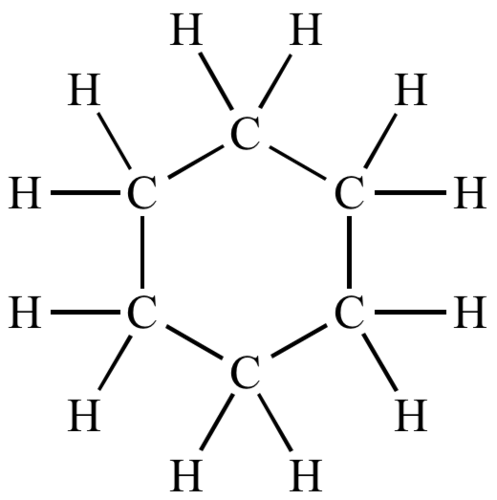
\includegraphics[width=.3\textwidth]{cyclohexane-500x500.png}
    \end{figure}
inside of the group $SO(2)$.
\item If we add the matrix
\[
[S] = \begin{pmatrix} 1 & 0 \\ 0 & -1 \end{pmatrix},
\]
then the group of matrices generated by $[R_\theta]$ and $[S]$ is the \boldblue{orthogonal group} $O(n)$. Argue that the dihedral group $D_n$ is a subgroup of $O(n)$.

\item What other symmetries of cyclohexane can you find that aren't inside of $SO(2)$? Are all of them in $O(n)$?
\end{enumerate}
\end{problem}

\begin{problem}{$U(1)$ and $SO(2)$}{}
The \boldblue{unitary group} $U(1)$ is the set of all $e^{i \theta}\in \C$ for $\theta \in [0,2\pi]$. In previous homework, we defined a map
\[
z=x+iy \mapsto [z] = x[I]+y[J].
\]
Show that this map applied to $U(1)$ yields an isomorphism to $SO(2)$, hence showing that there are equivalent representations of rotations in $\C$ and in $\R^2$.
\end{problem}


\subsection{Products of groups}
If groups are to represent symmetries, then we should be able to build new groups from old ones. Why is that? Well, take for example our square. From 6 squares glued along their edges, you can create a cube. This cube now has many more symmetry actions associated to it. For example, each face has the symmetries of a square, so there should be at least 6 copies of $C_4$ hiding within the symmetries of the cube. More formally:

\begin{definition}
Let $G$ and $H$ be groups, then we can form a new group $G\times H$ called the \boldblue{direct product}. Given $g_1,g_2 \in G$ and $h_1,h_2\in H$, we have elements $(g_1,h_1) \in G\times H$ and $(g_2,h_2)\in G\times H$ and the product is
\[
(g_1,h_1)(g_2,h_2) = (g_1g_2,h_1h_2).
\]
\end{definition}

\begin{example}
    Let us consider two groups $G=C_2$ and $H=C_4$. That is,
    \[
        G=\langle g~\vert~ g^2=e \rangle, \qquad H=\langle h ~\vert~ h^4=e \rangle.
    \]
    You can think of $G$ as the symmetries of a line segment and $H$ as the rotational symmetries of a square. Now, their direct product is the group $G\times H$. All of the elements in $G\times H$ are
    \begin{align*}
    (e,e), && (e,h) && (e,h^2) && (e,h^3)\\
    (g,e), && (g,h) && (g,h^2) && (g,h^3).
    \end{align*}
If you'd like, you can picture this as the group of symmetries of a square that is attached to the end of a line segment, i.e., a square shaped lollipop.
\end{example}

\begin{example}
    If we took instead $G=C_2$ and $H=C_2$ then we have a different group. This is the symmetries of two different line segments attached together. We have
    \[
        G=\langle g~\vert~ g^2=e \rangle, \qquad H=\langle h ~\vert~ h^2=e \rangle,
    \]
    so the list of elements is
    \begin{align*}
    (e,e), && (e,h)\\
    (g,e), && (g,h).
    \end{align*}
    The group $C_2 \times C_2$ are the symmetries of the rectangle! Often this is written as $V_4 \coloneqq C_2\times C_2$ and is called the \boldblue{Klein 4-group}.
\end{example}

\begin{problem}{Multiplication Table}{}
Write out the multiplication table for $C_2 \times C_2$.
\end{problem}

\begin{problem}{$\R^2=\R\times \R$}{}
Show that the group (vector space) $\R^2$ is equivalent to the group $\R\times \R$. Then argue that $\R^n = \underbrace{\R\times \R \times \cdots \R}_{\textrm{$n$ times}}$.
\end{problem}

\subsection{Formal Statement about Symmetries}

Just to cap this section off, I'd like to show you the theorem that states that all groups really are symmetries of some set. In fact, they're symmetries of themselves. The other fact that the symmetries of an object form a group (which we briefly argued) shows that groups and symmetries are interchangeable. Here's the theorem:

\begin{theorem}[Cayley's Theorem]
    Let $G$ be a group. Then $G$ is a subset of the of the symmetric group on the elements of $G$ which we write as $\mathrm{Sym}(G)$.
\end{theorem}

The meaning of this is as follows. We built up the idea of symmetry actions, and if we create some group $G$, it must be that it is built out of symmetry actions on itself. Just for grins, let's see another application of group theory.

\begin{problem}{Rubik's Cube}{}
Read some of this Wikipedia page: \url{https://en.wikipedia.org/wiki/Rubik%27s_Cube_group}. Write down something interesting that you learn from it.
\end{problem}

\section{Differential Equations}

Not all symmetries come about as symmetries of physical objects. For example, certain physical systems have some type of symmetry to them as well. For example, when we studied ODEs we discussed the idea that $x(t)$ can be thought of as modeling the state of the system over time $t$. At another time $x(\tau)$, this should also represent a valid state of the system. Thinking of this more abstractly now, $x\colon \R \to M$ where $M$ is some set. For example, take $M=(0,\infty)$ as well and make the assertion that $x$ satisfies some type of natural law such as $\frac{d}{dt}x = x$ under a further constraint that $x(0)=1$. Then $x$ is a group homomorphism. How so? First, note that $(0,\infty)$ is a group under multiplication (since we are not including 0).
\begin{problem}{}{}
Quickly explain how $(0,\infty)$ is a group under multiplication. What are the inverses?
\end{problem}

Then note that the solution to this IVP is $x(t)=e^t$ and so to be a homomorphism we must have
\[
x(t+\tau) = e^{t+\tau} = e^t e^\tau = x(t)x(\tau).
\]
Since we wrote the product as $+$, we must realize that the product in the image is now multiplication. But this is almost tautological. The exponential function is exactly the function for which associates a product with addition, e.g., $b^xb^y = b^{x+y}$. Our physical system which we built is equivalent to a requirement that we just want a homomorphism out of the abelian group $\R$ into some new set. In this case, it just so happens the new set is a group equal to the image $x(\R)$, but the new set could be something just containing this image. Finally, we can realize we asserted some of this here -- we took $x(0)=1$ and forced $x$ to take the identity $0$ of $\R$ to the identity 1 of $(0,\infty)$. If this was not the case, the group structure becomes less obvious, but it is still there./

This is rather miraculous, isn't it? Somehow, all along, this highly symmetric physical system whose derivative was itself corresponds to a group structure. This is, in some sense, true for all dynamical systems. They are seen as homomorphisms from $\Z$ if they are discrete time systems, $\R$ if they are causal ODEs. If they are periodic, then they are maps from the circle group $S^1$, but we will save this idea for another day.

In fact, a much bigger result is the following. Note that I have adjusted the statement to be more suitable for all of us.

\begin{theorem}[Emmy Noether's Theorem]
Every symmetry of a system corresponds to a conserved quantity of the system.
\end{theorem}

\begin{problem}{Emmy Noether}{}
Read some of the Wikipedia page about Emmy Noether: \url{https://en.wikipedia.org/wiki/Emmy_Noether}. Write down something interesting other than the fact that many other mathematicians and scientists including Einstein thought she was the most important woman in the history of mathematics.
\end{problem}

\begin{problem}{Energetics}{}
Consider the harmonic oscillator equation
\[\
mx'' + k x = 0.
\]
We note that this equation is a second order, linear, homogeneous, and, most importantly, autonomous equation.
\begin{enumerate}[(a)]
    \item Noting that the force $F=ma=mx''$, argue that the force itself is independent of time $t$. This is a symmetry in time.
    \item Write down the general solution to this equation.
    \item Corresponding to the time symmetry, energy must be conserved. This is because $t$ and $E$ are conjugate variables as position $x$ and momentum $p$ are as well. To this end, show
    \[
    E = \frac{1}{2}mx'^2 + \frac{1}{2}kx^2,
    \]
    is constant in time.
    \item You have shown that if $x$ is a solution to the Hamilton equation
    \[
    x'=ix,
    \]
    then $x$ is a solution to the harmonic oscillator equation (for the correct choices of $m$ and $k$). If we require as well $x(0)=1$, then show that $x$ is a homomorphism from $\R$ to the unitary group $U(1)$.
    \item Can you argue that the groups $(0,\infty)$ and $U(1)$ are not isomorphic? Can you see how the additional $i$ added to the equation changes the symmetries of the problem?
\end{enumerate}
\end{problem}

\section{Conclusions}

Group theory is a massive subject. Massive, yet it talks about something so simple: a set with an invertible binary operation. I hope that this project was challenging, but rewarding. I hope that you have found at least something in working through this interesting. There's many places this can go, and there are many reasons to study group theory. I did my best to grab enough but not too many of the basic ideas and give you problems that could work through and learn something from. I especially wanted you to realize that the concepts are useful in the real world as well. Just two more questions to go.

\begin{problem}{}{}
What else would you have liked to learn about group theory? What parts of this project worked well, and what parts didn't?
\end{problem}

One thing I would have liked to include is the idea of quotienting groups. This would have given us the understanding of how adding geometric restrictions gives you a quotient group.

\begin{problem}{}{}
Do you have any suggestions for Math 272? What can be done to make the class better for you? If you are not taking 272, then please still give me suggestions!
\end{problem}

\end{document}
